\documentclass{article}

\usepackage[margin=1in]{geometry}
\usepackage{amsmath,amsthm,amssymb}
\usepackage{bbm,enumerate,mathtools}
\usepackage[hidelinks]{hyperref}
\usepackage{tikz}
\usetikzlibrary{matrix, arrows}

\newenvironment{problem}[2][Problem]{\begin{trivlist}
\item[\hskip \labelsep {\bfseries #1}\hskip \labelsep {\bfseries #2.}]}{\end{trivlist}}
\newenvironment{solution}[1][Solution.]{\begin{trivlist}
\item[\hskip \labelsep {\bfseries #1}]}{\end{trivlist}}
\newenvironment{problempart}[1]{\begin{trivlist}\item[\textbf{Part #1.}]}{\end{trivlist}}

\begin{document}

\title{Combinatorics: Homework 7}
\author{Peter Kagey}

\maketitle

% -----------------------------------------------------
% First problem
% -----------------------------------------------------
\begin{problem}{21 (a)} $[2+]$ \\
  Given numbers $a_i$ for $i \in \mathbb Z$, with $a_i = 0$ for $i < 0$ and
  $a_0 = 1$, let $f(k) = \det[a_{j-i+1}]_1^k$. In particular, $f(0) = 1$. Show
  that \[
    \sum_{k \geq 0} f(k)x^k = \frac{1}{1 - a_1x + a_2x^2 - \cdots}.
  \]
\end{problem}

\begin{solution} \text{}
  % \[
  %   \begin{bmatrix}
  %        a_1 &    a_2 &    a_3 &    a_4 & \hdots & a_x &  a_k \\
  %          1 &    a_1 &    a_2 &    a_3 & \hdots & a_x &  a_{k - 1}\\
  %          0 &      1 &    a_1 &    a_2 & \hdots & a_x &  a_{k - 2}\\
  %          0 &      0 &      1 &    a_1 & \hdots & a_x &  a_{k - 2}\\
  %          0 &      0 &      0 &      1 & \hdots & a_x &  a_{k - 2}\\
  %     \vdots & \vdots & \vdots &        & \ddots & \ddots & \vdots \\
  %          0 &      0 &      0 &      0 & \hdots &   1 &  a_1 \\
  %   \end{bmatrix}
  % \]
  % By induction, using the Laplace expansion, \[
  %   f(k) = a_1f(k - 1) - \begin{vmatrix}
  %        a_2 &    a_3 &    a_4 & \hdots & a_x &  a_k \\
  %          1 &    a_1 &    a_2 & \hdots & a_x &  a_{k - 2}\\
  %          0 &      1 &    a_1 & \hdots & a_x &  a_{k - 2}\\
  %          0 &      0 &      1 & \hdots & a_x &  a_{k - 2}\\
  %     \vdots & \vdots &        & \ddots & \ddots & \vdots \\
  %           0 &      0 &      0 & \hdots &   1 &  a_1 \\
  %   \end{vmatrix}
  % \]
  It is sufficient to show that \begin{align*}
    1
    &= (1 - a_1x + a_2x^2 - \cdots)\sum_{k \geq 0} f(k)x^k \\
    &= \left(\sum_{n \geq 0} (-1)^n a_n x^n\right)\left(\sum_{k \geq 0} f(k)x^k\right) \\
    &= \sum_{n,k \geq 0} (-1)^n a_n f(k)x^{n+k}.
  \end{align*}
  This means is enough to show that the coefficient of $x^m$ is zero for all $m > 0$: \begin{align*}
    0  &= \sum_{i=0}^m (-1)^i a_i f(m-i) \\
    f(m) & = \sum_{i=1}^m (-1)^{i-1} a_i f(m-i) \\
    f(m) & = a_1f(m-1) - a_2f(m-2) + a_3f(m-3) + \hdots + (-1)^{m-1} a_m\underbrace{f(0)}_{=1}.
  \end{align*}
  This can be shown by Laplace expansion along the first row.
  Notice that $f(k) = \sum_{i=1}^k (-1)^{i-1} a_i \det(M_i)$ where $M_i$ is the
  $k-1 \times k-1$ submatrix illustrated below.
  \\
  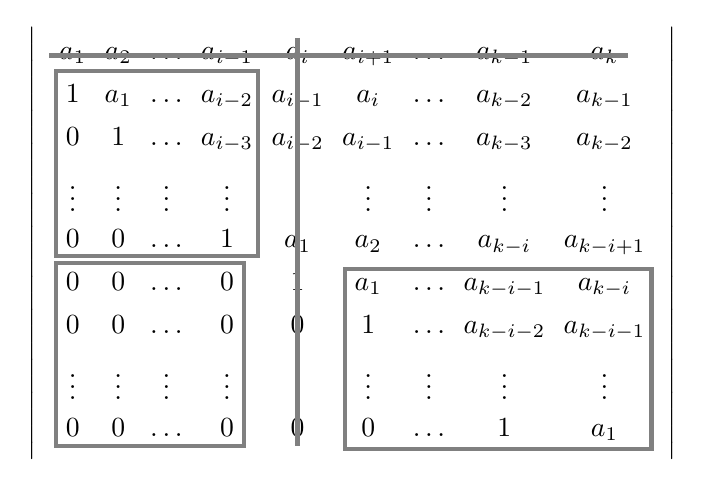
\begin{tikzpicture}
     \matrix (mat) [%
       matrix of nodes,
       left delimiter={|},right delimiter={|}
     ]
      {%
        $a_1$ & $a_2$ & $\hdots$ & $a_{i-1}$ & $a_{i}$ & $a_{i+1}$ & $\hdots$ & $a_{k-1}$ & $a_k$\\
        $1$ & $a_1$ & $\hdots$ & $a_{i-2}$ & $a_{i-1}$ & $a_{i}$ & $\hdots$ & $a_{k-2}$ & $a_{k-1}$\\
        $0$ & $1$ & $\hdots$ & $a_{i-3}$ & $a_{i-2}$ & $a_{i-1}$ & $\hdots$ & $a_{k-3}$ & $a_{k-2}$\\
        $\vdots$ & $\vdots$ & $\vdots$ & $\vdots$ & $\vdots$ & $\vdots$ & $\vdots$ & $\vdots$ & $\vdots$\\
        $0$ & $0$ & $\hdots$ & $1$ & $a_1$ & $a_2$ & $\hdots$ & $a_{k-i}$ & $a_{k-i+1}$\\
        $0$ & $0$ & $\hdots$ & $0$ & $1$ & $a_1$ & $\hdots$ & $a_{k-i-1}$ & $a_{k-i}$\\
        $0$ & $0$ & $\hdots$ & $0$ & $0$ & $1$ & $\hdots$ & $a_{k-i-2}$ & $a_{k-i-1}$\\
        $\vdots$ & $\vdots$ & $\vdots$ & $\vdots$ & $\vdots$ & $\vdots$ & $\vdots$ & $\vdots$ & $\vdots$\\
        $0$ & $0$ & $\hdots$ & $0$ & $0$ & $0$ & $\hdots$ & $1$ & $a_{1}$\\
      };
      \draw[gray, ultra thick] (mat-1-1.west)  -- (mat-1-9.east);
      \draw[gray, ultra thick] (mat-1-5.north) -- (mat-9-5.south);

      \draw[gray, ultra thick] (-3.76, 2.2) rectangle (-1.2,-0.15);
      \draw[gray, ultra thick] (mat-6-1.north west) rectangle (mat-9-4.south east);
      \draw[gray, ultra thick] (mat-6-6.north west) rectangle (3.8, -2.6);
  \end{tikzpicture}
  \\
  In particular, the structure of this matrix is \begin{itemize}
    \item the $f(k-i)$ matrix in the bottom $k-i$ rows and right $k-i$ columns,
    \item an upper triangular matrix in the top $i-1$ rows and left $i - 1$ columns, and
    \item the zero matrix in the bottom $k-i$ rows and left $i-1$ columns.
  \end{itemize}
  Thus, the determinant of $M_i$ can be computed by Laplace expansion, along
  the $i-1$ upper-left $1$s, until the $f(k-i)$ matrix is reached.
  So \[
    f(m) = \sum_{i=1}^m (-1)^{i-1} a_i f(m-i)
  \] for all $m > 0$. Since $f(0) = 1$ when $m = 0$ (by hypothesis), the identity follows.
\end{solution}
\pagebreak
% -----------------------------------------------------
% Second problem
% -----------------------------------------------------
\begin{problem}{26} $[2+]$ \\
  Let $\pi \in \Pi_n$, the set of partitions of $[n]$. Let $S(\pi, r)$ denote
  the number of $\sigma \in \Pi_n$ such that $|\sigma| = r$ and
  $\#(A \cap B) \leq 1$ for all $A \in \pi$ and $B \in \sigma$.
  Show that \[
    S(\pi, r) =
    \frac{1}{r!}\sum_{i=0}^r \binom ri (-1)^{r-i}\prod_{A \in \pi} (i)_{\#A}.
  \]
\end{problem}

\begin{solution} \text{} \\
  This can be counted with straightforward Inclusion-Exclusion.
  We will count the number of ordered partitions, and then divide by $r!$ to
  get unordered partitions.
  \\~\\
  We will first count the number of ways to partition $[n]$ into $r$-tuples
  that meet the above criteria \textit{and where some of the parts can be empty}.
  \\
  For sake of convenience, order $\pi$ in the canonical way. Then the first
  element of the first set of $\pi$ can go in any of the $r$ ``slots'', because
  $\#(A \cap B) \leq 1$, the second element of the first set of $\pi$ can go in
  $r - 1$ slots, the $k$th in $r - k + 1$. Thus the number of choices for the
  first set $A \in \pi$ is $(i)_{\#A}$.
  \\~\\
  We can do a similar argument for the remaining sets in $\pi$, resulting in
  \[
    \prod_{A \in \pi} (r)_{\#A}
  \] possible tuples.
  However, as stated earlier, this includes $r$-tuples where some of the parts
  are empty. So we must subtract these off \[
    \prod_{A \in \pi} (r)_{\#A} - \binom r1\prod_{A \in \pi} (r - 1)_{\#A},
  \] where $\binom r1$ is the number of ways to choose the empty position.
  \\
  However, this subtracts off too many $r$-tuples. In particular, it
  double-counts those where two or more parts are empty, so we must add these
  back in, and so on by the Principle of Inclusion-Exclusion
  \[
    \prod_{A \in \pi} (r)_{\#A}
    - \binom{r}{1}\prod_{A \in \pi} (r - 1)_{\#A}
    + \binom{r}{2}\prod_{A \in \pi} (r - 2)_{\#A}
    + \hdots
    + \binom{r}{r}\prod_{A \in \pi} (0)_{\#A}
    = \sum_{i=0}^r \binom ri (-1)^{r-i}\prod_{A \in \pi} (i)_{\#A}.
  \]
  Lastly, since the parts of the $r$-tuple are distinct, we can divide by the
  number of permutations, so \[
    S(\pi, r) =
    \frac{1}{r!}\sum_{i=0}^r \binom ri (-1)^{r-i}\prod_{A \in \pi} (i)_{\#A},
  \] as desired.
\end{solution}
\pagebreak
% -----------------------------------------------------
% Third problem
% -----------------------------------------------------
\begin{problem}{3}
  Let $E_{2n}$ be the number of ``alternating'' permuations,
  $w \in S_{2n}$ such that \[
    w_1 > w_2 < w_3 > w_4 < \hdots > w_{2n}
  \]
  Show that \[
    \sum_n E_{2n}\frac{x^{2n}}{(2n)!}
    = \frac{1}{1 - x^2/2! + x^4/4! - x^6/6! + \hdots}
    = \frac{1}{\cos(x)}.
  \]
\end{problem}

\begin{proof} \text{} \\
  Using the technique from class, we'll instead count the case where each $<$
  is replaced with no relation. Then since the $<$ are at all even positions,
  we can write \[
    \underbrace{w_1 > w_2}_{s_1 = 2},
    \underbrace{w_3 > w_4}_{s_2 - s_1 = 2},
    \hdots
    \underbrace{w_{2n-1} > w_{2n}}_{s_n - s_{n-1} = 2}.
  \]
  In particular, $s_i - s_j$ = $2(j - i)$.
  So using the determinant technique: \[
    E_{2n} = (2n)! \begin{vmatrix}
      \frac{1}{s_1!} &    \frac{1}{s_2!}         & \frac{1}{s_3!}         & \hdots & \frac{1}{s_{n-1}!}         & \frac{1}{s_n!} \\
                   1 &    \frac{1}{(s_2 - s_1)!} & \frac{1}{(s_3 - s_1)!} & \hdots & \frac{1}{(s_{n-1} - s_1)!} & \frac{1}{(s_n - s_1)!}\\
                   0 &                         1 & \frac{1}{(s_3 - s_2)!} & \hdots & \frac{1}{(s_{n-1} - s_2)!} & \frac{1}{(s_n - s_2)!}\\
                   0 &                         0 & 1                      & \hdots & \frac{1}{(s_{n-1} - s_3)!} & \frac{1}{(s_n - s_3)!}\\
              \vdots &                    \vdots & \vdots                 & \ddots & \ddots                     & \vdots \\
                   0 &                         0 &                      0 & \hdots & 1                          & \frac{1}{(s_n - s_{n-1})!}\\
    \end{vmatrix}
    = (2n)! \begin{vmatrix}
      \frac{1}{2!} & \frac{1}{4!} & \frac{1}{6!}         & \hdots & \frac{1}{(2n-2)!}         & \frac{1}{(2n)!} \\
      1            & \frac{1}{2!} & \frac{1}{4!}         & \hdots & \frac{1}{(2n-4)!}         & \frac{1}{(2n-2)!} \\
      0            & 1            & \frac{1}{2!}         & \hdots & \frac{1}{(2n-6)!}         & \frac{1}{(2n-4)!} \\
      0            & 0            & 1                    & \hdots & \frac{1}{(2n-8)!}         & \frac{1}{(2n-6)!} \\
      \vdots       & \vdots       & \vdots               & \ddots & \ddots                    & \vdots \\
      0            & 0            & 0                    & \hdots & 1                         & \frac{1}{2!}\\
    \end{vmatrix}
  \]
  This satisfies the property in problem 1, namely
  $\displaystyle \frac{E_{2n}}{(2n)!} = \det[a_{j-i+1}]_1^n$ with \[
    a_i = \begin{cases}
      0 & i < 0 \\
      1 & i = 0 \\
      \displaystyle\frac{1}{(2i)!} & i > 0
    \end{cases}.
  \]
  Therefore substituting $x^2$ for $x$ in problem 1 yields \[
    \sum_n \frac{E_{2n}}{(2n)!}x^{2n}
    = \frac{1}{1 - (1/2!)x^2 + (1/4!)x^4 - (1/6!)x^6 + \hdots}
  \] as desired.
\end{proof}
\pagebreak
\end{document}
